\chapter{Desarrollo del proyecto}
\label{chap:desarrollo}

\lettrine{E}{n} este capítulo se describe el proceso de desarrollo del proyecto. Se parte de la especificación de requisitos y de los actores del sistema, se presenta la metodología de trabajo empleada y la planificación seguida, y se detalla la gestión de los archivos del proyecto. Finalmente, se enumeran los recursos hardware, software y humanos utilizados y se realiza una estimación de los costes del trabajo.

\section{Requisitos}
\label{sec:requisitos}

En esta sección se detallan los requisitos que debe cumplir el sistema, definiendo tanto los aspectos funcionales como los no funcionales que determinan su diseño y funcionamiento. La definición de los requisitos constituye una parte esencial en el desarrollo de cualquier sistema, pues garantiza que el resultado final se ajuste a las expectativas y necesidades planteadas en las fases iniciales del proyecto.

\subsection{Requisitos funcionales}

Los requisitos funcionales declaran el comportamiento y las acciones que debe ofrecer el sistema. Definen las funcionalidades que los usuarios esperan y que deben poder llevarse a cabo para cumplir con los objetivos planteados.

\begin{enumerate}
    \item \textbf{Configuración del entorno de carrera.} El sistema debe permitir indicar el número de coches, el número de raíles del circuito y el color de las etiquetas de cada vehículo, de forma que cada coche pueda identificarse de manera unívoca durante la detección y el seguimiento.
    
    \item \textbf{Captura y detección distribuida de la posición.} El sistema debe capturar y procesar en tiempo real las imágenes de múltiples cámaras, con o sin solapamiento entre sus campos de visión, detectando la posición de los coches mediante segmentación por color.
    
    \item \textbf{Control adaptativo de la velocidad.} El sistema debe aplicar un algoritmo que ajuste dinámicamente la velocidad de cada coche en función de su posición y de las características del circuito, buscando recorrer cada tramo a la máxima velocidad posible sin comprometer la estabilidad (sin salirse ni derrapar en las curvas).
     
    \item \textbf{Visualización y telemetría en tiempo real.} El sistema debe mostrar en tiempo real información de interés para el usuario, como las imágenes procesadas, la posición, la trayectoria seguida y los tiempos por vuelta. Recopilando además la telemetría temporal de cada etapa del procesamiento para su posterior analisis.
    
    \item \textbf{Detección del paso por meta y cálculo de tiempos.} El sistema debe detectar el paso de cada coche por la línea de meta y, a partir de ella, registrar y calcular el número de vueltas completadas así como el tiempo por vuelta.
    
    \item \textbf{Arquitectura distribuida sobre red local.} El sistema debe diseñarse como un conjunto de nodos distribuidos que cooperan a través de una red local (wifi o Ethernet), repartiendo entre distintas máquinas las tareas de captura, detección, control y actuación. La comunicación entre nodos debe realizarse mediante el intercambio de mensajes por la red, sin memoria compartida, de forma que el sistema pueda cubrir circuitos de mayor tamaño y no quede limitado por los recursos ni por el número de puertos de un único equipo.
\end{enumerate}

\subsection{Requisitos no funcionales}

Los requisitos no funcionales definen las condiciones bajo las que debe operar el sistema, incluyendo aspectos como el rendimiento, la escalabilidad, la robustez o la estructura del código. Aunque no describen funciones concretas, resultan esenciales para garantizar que el sistema sea estable, mantenible y adecuado para su propósito.

\begin{enumerate}
\item \textbf{Arquitectura modular y distribuida.} La lógica del sistema debe organizarse en nodos independientes con responsabilidades delimitadas (captura y detección, control por rail y actuación sobre el hardware), comunicados a través de la red, de forma que cada nodo pueda ejecutarse en una máquina distinta sin compartir estado en memoria.

\item \textbf{Escalabilidad.} La arquitectura debe permitir aumentar el número de cámaras, raíles y coches, así como cubrir circuitos de mayor tamaño y complejidad, añadiendo nuevos nodos a la red sin necesidad de rediseñar el sistema.

\item \textbf{Robustez y tolerancia a perturbaciones.} El sistema debe mantener un funcionamiento estable ante fallos temporales, oclusiones o perturbaciones, como cambios en la orientación de las cámaras, recuperándose de forma automática siempre que sea posible.

\item \textbf{Sencillez en el despliegue} El despliegue del sistema debe ser reproducible empaquetando cada nodo y sus dependencias mediante contenedores, de modo que pueda instalarse y ejecutarse de forma consistente en distintas máquinas.
\end{enumerate}

\section{Actores}
\label{sec:actores}

El único actor que interviene es el \textbf{usuario final}, y su trabajo es previo a la carrera, ya que el sistema opera de forma autónoma una vez puesto en marcha. A diferencia de los trabajos anteriores, en los que se manejaba todo desde una aplicación de escritorio, aquí lo que decide el usuario es el despliegue, esto es, cuántos nodos cámara hacen falta para cubrir el circuito y en qué máquina se ejecuta cada nodo. Con eso decidido, ajusta el fichero de parámetros (los colores de las pegatinas de cada coche y de la línea de meta, los coches que participan o la resolución de las cámaras) y arranca un contenedor en cada equipo, tras lo cual los nodos se descubren entre ellos, calibran y empiezan a correr sin más intervención. Durante la carrera solo decide cuándo detenerla, aunque si lo desea puede seguirla desde el nodo de visualización, cambiar parámetros en caliente y, si guardó la información, analizar la sesión en diferido.

\section{Descripción del sistema}
\label{sec:descricion-sistema}

El sistema desarrollado es una plataforma distribuida para el control visual de coches de tipo Scalextric. A diferencia de la solución monolítica heredada, en la que todas las cámaras se conectaban físicamente a un mismo equipo, aquí la funcionalidad se reparte entre varios nodos que cooperan a través de una red local, cableada o inalámbrica, sobre ROS2 y su capa de mensajería publicador/suscriptor.

Son tres tipos de nodos. El \emph{nodo cámara}, uno por cada cámara física, captura los fotogramas, localiza en ellos las pegatinas de los coches y la línea de meta, y publica en la red la posición de cada vehículo. El \emph{nodo de control}, uno por cada carril por el que pueda circular un coche, recibe esas posiciones y decide en cada momento qué valor de PWM hay que aplicar al carril. Y el \emph{nodo de potencia} recoge esos valores de la red y los traslada por el puerto serie a la placa Arduino que alimenta los carriles.

La parte hardware está constituida por la placa Elegoo Uno R3 y el módulo controlador L293D, que reciben los comandos del nodo de potencia y regulan la tensión de cada carril mediante señales PWM, controlando así la velocidad de los coches. El conjunto de nodos se distribuye entre los distintos equipos de cómputo disponibles, y se despliega de forma reproducible mediante contenedores Docker, lo que elimina la necesidad de instalar ROS2 o sus dependencias en cada máquina.

\section{Metodología de desarrollo}
\label{sec:metodoloxia}

Buena parte del sistema depende de cómo se comporta un coche sobre la pista, y eso no se puede prever. Esa fue la razón de no planificar el trabajo de una sola vez y de repartirlo en entregas pequeñas que se llevaban a la pista en cuanto estaban listas. El punto de partida fue estudiar los TFG anteriores, localizar en ellos lo que había que mejorar y elegir las tecnologías con las que hacerlo. A partir de ahí se diseñó la arquitectura y se fue construyendo pieza a pieza, probando cada una sobre el circuito, y el trabajo se cerró con la memoria y la preparación de la defensa.

El desarrollo se organizó en iteraciones cortas, cada una orientada a incorporar una capacidad concreta al sistema. Una iteración no se daba por cerrada hasta validar su resultado sobre el hardware, de modo que las pruebas de cada etapa condicionaban el diseño de la siguiente.

Esta forma de trabajar sigue la filosofía de las metodologías ágiles, con entregas pequeñas y un replanteamiento continuo a la vista de lo aprendido en cada prueba, pero no se adoptó ningún marco concreto como Scrum, Kanban o programación extrema. Sus roles y ceremonias están pensados para coordinar a un equipo y, en un proyecto de una sola persona y de unos meses de duración, añaden más carga de la que aportan. El seguimiento se resolvió con reuniones periódicas con los tutores, en las que se revisaba la iteración en curso y se acordaban los objetivos de la siguiente. El código se llevó con Git desde el principio (sección~\ref{sec:xestion-arquivos}), etiquetando el mensaje de cada \textit{commit} según la funcionalidad que se estaba diseñando, de manera que el propio historial permite reconstruir por dónde fue avanzando el trabajo.

\section{Planificación e iteraciones}
\label{sec:planificacion-iteraciones}

De acuerdo con la metodología ágil e incremental descrita en la sección anterior, el desarrollo se estructuró en un conjunto de iteraciones cortas. Cada iteración persigue un objetivo concreto, incorpora una capacidad nueva al sistema y se cierra únicamente tras ser validada, de modo que los datos obtenidos en las pruebas realimentan el diseño de las siguientes etapas. El proceso avanza desde el estudio y análisis inicial hasta las pruebas finales del sistema completo, siguiendo el orden que se detalla a continuación.

\begin{itemize}

    \item \textbf{Iteración 1. Análisis inicial del proyecto.} Lectura y estudio de los TFG previos para entender el proyecto y para detectar partes de mejora. Además se definieron los objetivos y requisitos concretos de este trabajo. Se analizaron las tecnologías y herramientas disponibles, sobre todo qué protocolo de red resultaba más adecuado para dar soporte a la arquitectura que queríamos diseñar, dado que todo el sistema se sustenta en el intercambio de información a través de la red. De este estudio derivó la elección de ROS2 y su capa de comunicación basada en el middleware DDS. Pesaron también otros tres motivos. El primero es que se trata de un estándar en el desarrollo de aplicaciones de robótica, lo que facilita que el trabajo pueda retomarse más adelante para añadirle nuevas funcionalidades. El segundo es que trae ya resueltas y configuradas muchas herramientas de uso habitual, como la grabación de los datos o la gestión de la configuración, que de otro modo habría que programar. Y el tercero es que su modelo de comunicación publicador/suscriptor encajaba de forma natural con el diseño que se quería construir.

    \item \textbf{Iteración 2. Diseño de la arquitectura distribuida.} Diseño de la arquitectura del sistema y de la descomposición de la arquitectura monolítica planteada en trabajos anteriores en nodos independientes. El reto principal de esta fase fue afrontar el cambio de paradigma, ya que normalmente, en una arquitectura monolítica los distintos componentes comparten un mismo estado en memoria en cambio en un sistema distribuido esa información debe intercambiarse a través de la red. Esta limitación condiciona el diseño, ya que no toda la información puede consultarse ni intercambiarse de forma continua, y obliga a decidir qué datos se publican, con qué frecuencia y con qué garantías de entrega. Se definieron así los nodos del sistema, los mensajes que intercambian y las políticas de calidad de servicio (QoS) asociadas a cada flujo de datos.

    \item \textbf{Iteración 3. Detección de etiquetas y seguimiento de objetos.} Una vez decidido el diseño, se comenzó por el nodo cámara con un programa sencillo capaz de leer los fotogramas de una cámara y detectar las dos pegatinas de color del coche mediante filtros de color, obteniendo su posición dentro de la imagen. Esta iteración sienta la base del sistema de captura y detección sobre la que se construye el resto del sistema.

    \item \textbf{Iteración 4. Integración con la red.} Integración de ese primer nodo con la capa de comunicación de ROS2, con el fin de probar el envío de mensajes y imágenes a través de la red. El objetivo era validar que la información detectada podía publicarse y recibirse correctamente entre máquinas distintas, comprobando el funcionamiento real del paradigma publicador/suscriptor sobre el que se apoya toda la arquitectura. Para comprobarlo se escribió un primer nodo muy sencillo, que se limitaba a suscribirse al tópico y guardar lo que le iba llegando.

    \item \textbf{Iteración 5. Pruebas de hardware.} La idea de partida era emplear hardware sencillo al que pudieran conectarse directamente las cámaras. En esta iteración se estudió si ese hardware era capaz de soportar la carga de capturar, procesar y segmentar por color los fotogramas manteniendo un rendimiento aceptable, evaluando así su viabilidad para el despliegue distribuido del sistema.

    \item \textbf{Iteración 6. Región de interés y readquisición del seguimiento.} Para mejorar el rendimiento se implementó una región de interés (ROI) que restringe la búsqueda de las etiquetas a la zona donde se espera encontrar el coche, reduciendo el área de procesamiento en cada fotograma. Junto a ella se desarrolló el mecanismo de readquisición, encargado de recuperar el seguimiento cuando se pierde de forma temporal, de manera que el sistema siga funcionando de forma robusta ante oclusiones o pérdidas momentáneas de visibilidad.

    \item \textbf{Iteración 7. Nodo de análisis y captura de telemetría.} Se creó un nodo que recibe y guarda todo lo que circula por la red, apoyándose en la herramienta de grabación de ROS2 (\emph{rosbag}). Con esa información almacenada se escribió después un script del que sacar las métricas de cada sesión y estudiar el comportamiento del sistema.

    \item \textbf{Iteración 8. Diseño del nodo controlador.} Diseño de un nuevo nodo controlador que implementa un algoritmo sencillo, capaz de controlar el coche del circuito de Scalextric a partir de las posiciones recibidas. Esta primera versión del controlador establece la base del sistema de control de velocidad que se refinaría en iteraciones posteriores.

    \item \textbf{Iteración 9. Revisión del código del Arduino.} Dado que el código de la aplicación del Arduino ya estaba implementado en trabajos previos, esta iteración consistió en revisar que todo siguiera funcionando correctamente, comprender en detalle el funcionamiento del código y comprobar su correcto comportamiento antes de integrarlo en la nueva arquitectura.

    \item \textbf{Iteración 10. Nodo de potencia e integración con el Arduino.} Creación del nodo de potencia encargado de centralizar la comunicación con el Arduino, conectándolo a la placa a través del puerto serie y verificando su funcionamiento dentro de la arquitectura distribuida completa, con esta iteración se cierra el control del sistema desde la detección visual hasta la actuación sobre la pista.

    \item \textbf{Iteración 11. Mejora del algoritmo y pruebas finales.} Mejora y adaptación del algoritmo de control a las situaciones propias del entorno real. Se analizaron los resultados, se anotaron las pruebas de funcionamiento y se llevaron a cabo las pruebas finales del sistema completo, validando su comportamiento de forma integral.

    \item \textbf{Iteración 12. Documentación y preparación de la defensa.} Redacción de la memoria del trabajo, elaboración de la guía de instalación, despliegue y uso del sistema, y organización del repositorio de código para facilitar su reutilización en trabajos posteriores. Finalmente, se preparó la presentación para la defensa del proyecto.

\end{itemize}

El reparto de estas iteraciones en el tiempo se recoge en la figura~\ref{fig:gantt-base}. El trabajo arrancó en la semana del 16 de febrero de 2026 y la planificación inicial cerraba la última iteración el 26 de junio, diecinueve semanas después, dejando la redacción de la memoria solapada con las pruebas finales del sistema.

\begin{figure}[tbp]
    \centering
    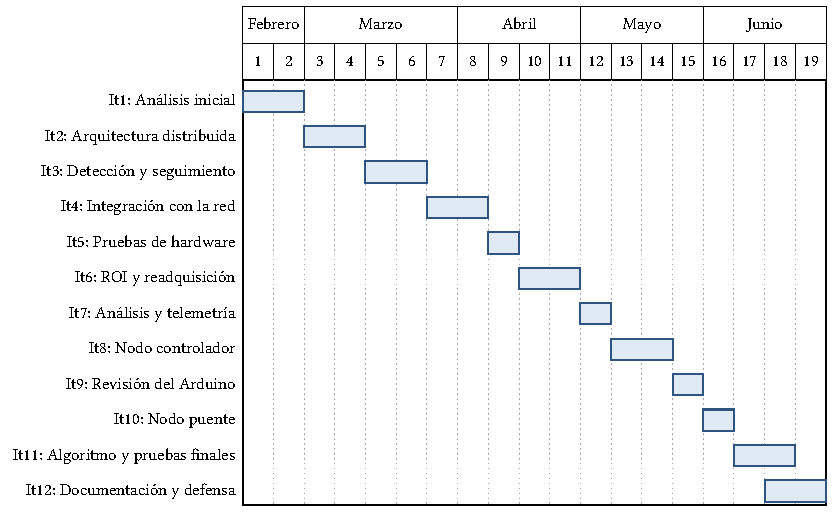
\includegraphics[width=0.8\textwidth]{imaxes/DESARROLLO/gantt_base.pdf}
    \caption{Planificación inicial del proyecto}
    \label{fig:gantt-base}
\end{figure}

A lo largo del proyecto surgieron diversas dificultades que condicionaron el ritmo del desarrollo. Las más relevantes se concentraron en la fase de integración con la red, donde el uso de Docker junto con ROS2 generó una serie de problemas que retrasaron el conseguir un despliegue estable. Asimismo, el hardware presentó fallos intermitentes que, al no manifestarse de forma constante, resultaron difíciles de diagnosticar y consumieron bastante tiempo. Finalmente, durante el desarrollo del algoritmo de control aparecieron fallos no previstos que obligaron a revisar y ajustar el diseño.

El efecto de esas dificultades sobre el calendario se ve en la figura~\ref{fig:gantt-retrasos}, que enfrenta cada iteración con la duración que tenía planificada. Las que más se alargaron fueron la integración con la red y la mejora del algoritmo, y por detrás las pruebas de hardware, mientras que las demás se desplazaron en bloque tras ellas, de forma que el trabajo se cerró siete semanas más tarde de lo previsto, a mediados de agosto, cambiando la fecha de entrega.

\begin{figure}[tbp]
    \centering
    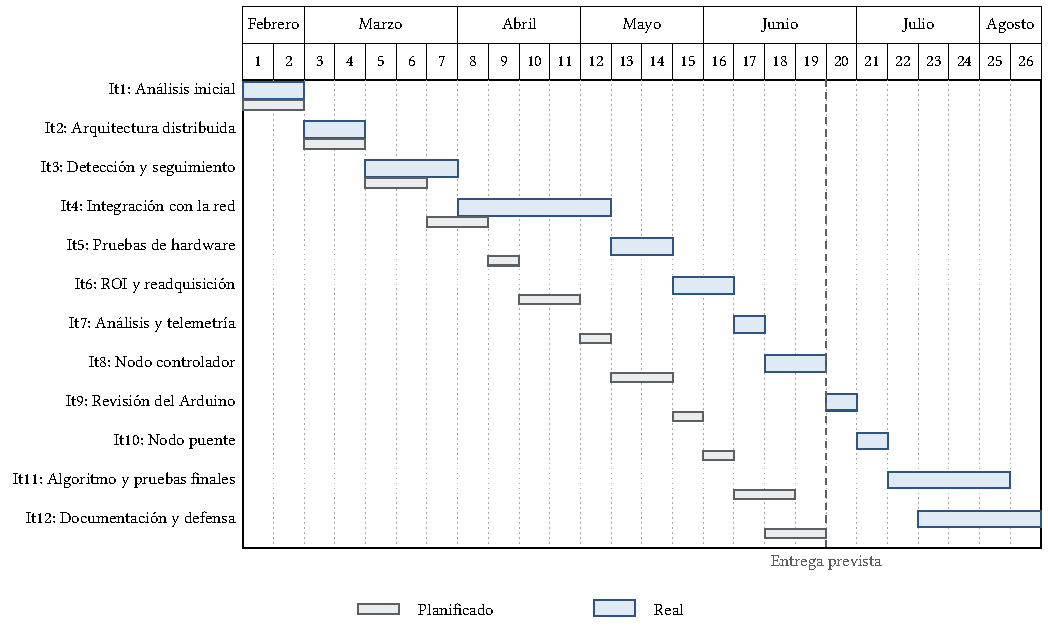
\includegraphics[width=\textwidth]{imaxes/DESARROLLO/gantt_retrasos.pdf}
    \caption{Planificación real del proyecto}
    \label{fig:gantt-retrasos}
\end{figure}


\section{Gestión de archivos}
\label{sec:xestion-arquivos}

Con el fin de garantizar la trazabilidad y la reproducibilidad del trabajo, todos los archivos generados durante el desarrollo del proyecto se han organizado y publicado en un repositorio de acceso público alojado en GitHub~\cite{repogithub}. Dicho repositorio reúne el código fuente de los nodos ROS2 escritos en Python, las definiciones de los mensajes personalizados intercambiados entre nodos, el firmware de Arduino encargado de generar las señales PWM, así como los ficheros de configuración del sistema (el fichero de parámetros en YAML y los ficheros de Docker Compose empleados en el despliegue).

Para ilustrar el funcionamiento del sistema se han grabado y publicado vídeos de las distintas pruebas realizadas, capturados a partir de las grabaciones (sección~\ref{sec:ros2-rosbag}) y accesibles desde el canal de YouTube asociado al proyecto~\cite{canalyoutube}. Este material aporta evidencia visual de los resultados alcanzados.

\section{Recursos}
\label{sec:recursos}

En esta sección se enumeran los recursos hardware, software y humanos que han intervenido en el desarrollo del proyecto.

\subsection{Recursos hardware}

El material empleado se agrupa en tres bloques. El primero es la pista, un circuito de Scalextric con la electrónica que le aplica la tensión, formada por la placa Elegoo Uno R3 y el módulo controlador L293D. El segundo es el equipamiento de visión, con cuatro cámaras web (dos Microsoft LifeCam HD-5000 y dos Logitech Brio 100) y dos placas Raspberry Pi 5, que son las que ejecutan los nodos de captura. El tercero es el ordenador portátil ASUS Vivobook S 14, donde se ejecutaban habitualmente los nodos de control y el nodo de potencia, por lo que es el que tenía la placa conectada por USB. Todo ello se detalla, junto con su coste, en la tabla~\ref{tab:costes_hardware} de la sección~\ref{sec:custos}.

\subsection{Recursos software}

Todo el software empleado en el proyecto es de código abierto o de uso gratuito, por lo que no lleva asociado ningún coste de licencia. El listado completo se detalla en el capítulo de tecnologías; los lenguajes de programación utilizados fueron:

\begin{itemize}
    \item Python, empleado en la implementación de los nodos ROS2 y de toda la lógica de visión y control.
    \item C/C++, utilizado en el firmware de la placa Arduino encargado de interpretar los comandos de velocidad y generar las señales PWM.
\end{itemize}

\subsection{Recursos humanos}

Durante el desarrollo del proyecto, el alumno ha asumido de forma íntegra los distintos roles que intervienen en un proceso de ingeniería del software:

\begin{itemize}
    \item \textbf{Jefe de proyecto}: planifica y coordina las fases del desarrollo y actúa como enlace con los tutores.
    \item \textbf{Analista}: recopila y modela los requisitos del sistema y define las especificaciones funcionales.
    \item \textbf{Arquitecto de software}: diseña la arquitectura distribuida, selecciona las tecnologías y establece la estructura modular basada en nodos.
    \item \textbf{Programador}: implementa las funcionalidades, integra los distintos nodos y realiza tareas de optimización.
    \item \textbf{Responsable de pruebas}: diseña y ejecuta las pruebas necesarias para verificar el correcto funcionamiento del sistema.
\end{itemize}

\section{Estimación de costes}
\label{sec:custos}

En este apartado se estima el coste total del proyecto a partir de los recursos materiales y humanos empleados. Los recursos software no generan coste alguno, ya que todo el software utilizado es libre o gratuito.

El coste de los recursos hardware se recoge en la tabla~\ref{tab:costes_hardware}. Todo el material aparece a precio de compra salvo el ordenador portátil, que no se adquirió para este trabajo, sino que es un equipo personal empleado también para otras tareas. Su coste se estima por amortización, repartiendo los 1.600~\euro{} que costó entre una vida útil de cuatro años, lo que supone 1,10~\euro{} al día y un total de 197~\euro{} por los 180 días que duró el desarrollo.

\begin{table}[tbp]
    \centering
    \estilotabla
    \caption{Costes derivados del hardware}
    \label{tab:costes_hardware}
    \begin{tabular}{lc}
        \toprule
        \rowcolor{ArqAzulClaro}
        \textbf{Dispositivo} & \textbf{Coste} \\
        \midrule
        Elegoo Uno R3                         & 19,99 \euro   \\
        Controlador de Motores L293D          & 5,81 \euro    \\
        Microsoft LifeCam HD-5000 ($\times$2) & 70,42 \euro   \\
        Logitech Brio 100 ($\times$2)         & 80,00 \euro   \\
        Circuito Scalextric EVOLUTION         & 119,99 \euro  \\
        Raspberry Pi 5 ($\times$2)            & 180,00 \euro  \\
        Router TP-Link Archer AX55            & 89,99 \euro   \\
        Adaptador de red Archer T3U ($\times$2) & 39,98 \euro \\
        ASUS Vivobook S 14 (amortización)     & 197,00 \euro  \\
        \midrule
        \textbf{Total} & \textbf{803,18 \euro} \\
        \bottomrule
    \end{tabular}
\end{table}

Respecto a los recursos humanos, el desarrollo se llevó a cabo a lo largo de aproximadamente 180 días, con una dedicación media en torno a las 3 horas diarias, aunque hubo días de un periodo mayor y otros en los que hubo menos, lo que supone un total cercano a las 540 horas de trabajo efectivas. El esfuerzo se distribuyó entre los distintos roles asignando a cada uno una carga horaria acorde con sus responsabilidades, concentrándose la mayor parte del tiempo en las tareas de programación. El desglose de horas y costes se muestra en la tabla~\ref{tab:costes_humanos}.

\begin{table}[tbp]
    \centering
    \estilotabla
    \caption{Desglose de horas y costes de los recursos humanos}
    \label{tab:costes_humanos}
    \begin{tabular}{lccc}
        \toprule
        \rowcolor{ArqAzulClaro}
        \textbf{Rol} & \textbf{Horas} &
        \textbf{Coste/hora (\euro/h)} & \textbf{Coste total (\euro)} \\
        \midrule
        Jefe de proyecto        & 55  & 60 & 3\,300  \\
        Analista                & 45  & 45 & 2\,025  \\
        Arquitecto de software  & 50  & 55 & 2\,750  \\
        Programador             & 320 & 50 & 16\,000 \\
        Responsable de pruebas  & 35  & 40 & 1\,400  \\
        Documentador            & 35  & 40 & 1\,400  \\
        \midrule
        \textbf{Total} & \textbf{540} & --- & \textbf{26\,875} \\
        \bottomrule
    \end{tabular}
\end{table}

Sumando el coste de los recursos hardware (tabla~\ref{tab:costes_hardware}) y el de los recursos humanos (tabla~\ref{tab:costes_humanos}), y teniendo en cuenta que los recursos software no suponen coste alguno, el coste total estimado del proyecto asciende a \textbf{27\,481{,}18 \euro}.